\documentclass[11pt, letterpaper]{article}

\usepackage[margin=1in]{geometry}
\usepackage{graphicx}
\usepackage{float}
\usepackage{booktabs}
\usepackage{hyperref}
\usepackage{setspace}
\usepackage{parskip}
\usepackage{titlesec}
\usepackage[T1]{fontenc}
\usepackage[utf8]{inputenc}

\graphicspath{{figures/}}

\titleformat{\section}{\large\bfseries}{}{0em}{}[\titlerule]
\titleformat{\subsection}{\normalsize\bfseries}{}{0em}{}

\title{\textbf{Executive Summary}\\[0.5em]
\large Transit Proximity and Gentrification Risk Along the D Line Extension}
\date{\today}
\author{Team: Ride the D(Line)}
\begin{document}

\maketitle
\thispagestyle{empty}

\tableofcontents

\section{Background (Judith)}

Los Angeles is extending its metro rail with the D Line, and transit proximity is routinely marketed
as a neighborhood amenity. That same amenity has coincided with rising rents and displacement along
earlier rail expansions across the city. With 63\% of Angelenos renting, a shift in housing costs
reaches most of the population, not a narrow slice of it. The question this analysis takes up is
where, along the new corridor, that pressure is most likely to land.

\section{Approach (Jon)}

The analysis combined listing-level rental data with ZIP-level demographic and housing measures and
the geographic locations of existing and planned Metro stops, covering roughly 15,700 listings within
five miles of a station. From these inputs we built a composite gentrification risk score (CGRS) that
captures five distinct signals of displacement pressure: rent premium (how far a listing's price sits
above the local median), rent burden (rent measured against what a median-income household can
afford), spatial rent appreciation (rent growth from 2019 to 2024), price per square foot premium
(the cost of space itself, adjusted for unit size), and education change (the shift in college-degree
share over the same window). Each component is z-scored and averaged with equal weight, so the final
CGRS places every listing on a common scale where zero is the average and positive values indicate
above-average risk.

We then measured how that risk relates to distance from Metro stops, testing whether listings closer
to transit carry systematically different risk than those farther away. To forecast the D Line, we
trained a set of models (linear, ridge, random forest, and gradient-boosted trees) and used the
random forest, restricted to the A and E Line corridors, because those lines most resemble the D Line
in density and income mix. Because three of the five components are point-in-time measures, the CGRS
describes current pressure more than long-run change, though the two trajectory measures (rent
appreciation and education change) let it pick up neighborhoods in early transition.

\section{Key Findings (Daniel)}


Transit is supposed to lift the neighborhood it serves. Along the D Line, the biggest displacement
risk sits one neighborhood over. Our analysis predicts little to no added pressure in the Westwood
and UCLA corridor, and that is not because the area is shielded. Rents there have already topped
out, with little room left to climb. The pressure does not disappear. It shifts to still-affordable
areas like Koreatown, Palms, and Mar Vista, which carry the highest composite gentrification risk
along the line.

\begin{figure}[H]
    \centering
    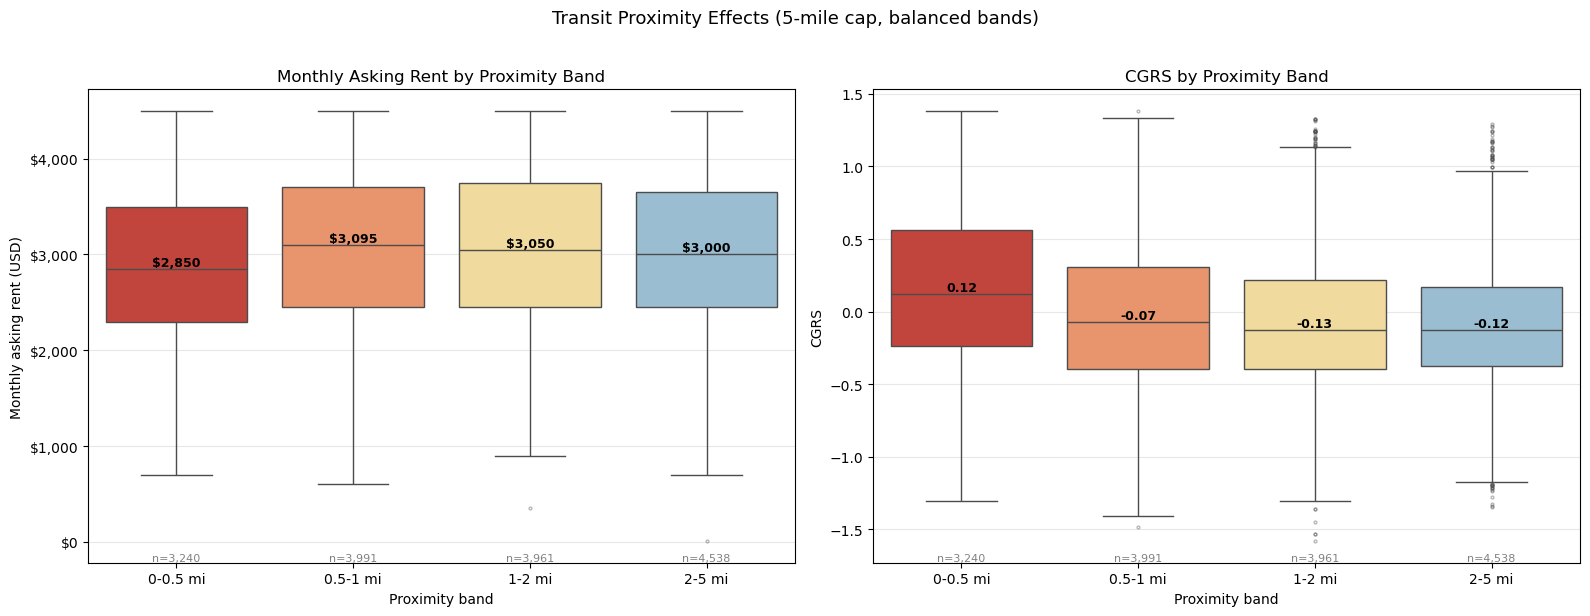
\includegraphics[width=\textwidth]{eda_band_boxplots.png}
    \caption{Monthly asking rent (left) and CGRS (right) by proximity band. Listings within
    0.5~miles of a station post the lowest median rent (\$2,850) yet the highest median CGRS
    (0.12), while all bands beyond 0.5~miles show negative median CGRS values, consistent with
    the transit-proximity effect documented in the analysis.}
\end{figure}

The pattern in the data is consistent. Listings within a half mile of a Metro station carried a
median risk score of 0.125, compared to $-0.112$ for listings farther out, a gap that holds up
under a one-sided Mann-Whitney U test ($p < 0.001$). Mean risk also falls steadily as distance to
the nearest station grows, so proximity and gentrification pressure track together across the sample
rather than at a single cutoff.

\begin{figure}[H]
    \centering
    
\includegraphics[width=0.8\textwidth]{eda_distance_decay.png}
    \caption{Distance-decay of gentrification risk. Each point is an individual listing; the red
    line traces the bin-mean CGRS. Risk is highest immediately adjacent to stations and declines
    monotonically through the first $\sim$2~km before stabilising.}
\end{figure}

Risk levels differ sharply from one Metro line to the next as well (Kruskal-Wallis $p < 0.001$),
which is why the forecast trains on the corridors most like the D Line rather than the full network.

To project the extension, we ran each listing through the model twice, once at its real distance
from transit and once as if a station sat within walking range, then took the difference as the
added pressure attributable to the new stations. In Westwood and UCLA that difference is near zero. The corridor's baseline risk is already high, so
the stations arrive into a market that has mostly priced in the change. The open question is not
whether transit access raises the cost of the corridor it serves. Here, that corridor has already
topped out. It is what happens to the affordable neighborhoods sitting just beyond it.


\section{What This Does and Does Not Show (Layla)}

These findings should be read as an association, not a cause. The analysis is cross-sectional, so it
captures a single moment and cannot show how risk will shift as transit access expands. It also
cannot separate the Metro's influence from the fact that LA's rail already runs through some of the
city's most established corridors. Proximity may reflect where high-value neighborhoods already sit,
or it may be an early signal of pressure that has not yet surfaced. The results point to a pattern
worth watching closely, not a confirmed effect.

\end{document}
